\documentclass[12pt]{article}
\usepackage{amsfonts}
\usepackage{fancyhdr}
\usepackage{comment}
\usepackage[a4paper, top=1cm, bottom=1.5cm, left=2cm, right=2cm]{geometry}
\usepackage{enumitem}
\usepackage{times}
\usepackage{changepage}
\usepackage{amssymb}
\usepackage{graphicx}
\usepackage{tabularx}
\usepackage{titlesec}
\usepackage{changepage}
\usepackage[parfill]{parskip}
\usepackage{wrapfig}
\usepackage[export]{adjustbox}
\usepackage{multirow}
\usepackage{array}
\usepackage[table]{xcolor}
\usepackage{longtable,booktabs}
\usepackage{float}
\usepackage{listings} % For presenting code nicely
\usepackage{hyperref}
\usepackage{framed}

\hypersetup{
    colorlinks,
    citecolor=black,
    filecolor=black,
    linkcolor=black,
    urlcolor=black
}

% settings %
\setcounter{secnumdepth}{2} % enumerate
\setcounter{tocdepth}{2}    % TOC entries
%\renewcommand{\contentsname}{Innholdsfortegnelse}
\newcounter{frcounter}
\newcounter{frsubcounter}[frcounter]
\newcounter{nfrcounter}
\newcounter{nfrsubcounter}[nfrcounter]
\titlespacing*{\paragraph}{\parindent}{1ex}{1em}

% commands %
    % counters %
\newcommand*{\FR}{\stepcounter{frcounter}\textbf{[FR-\arabic{frcounter}] \quad}}
\newcommand*{\FRsub}{\stepcounter{frsubcounter}\textbf{[FR-\arabic{frcounter}.\arabic{frsubcounter}] \quad}}
\newcommand*{\NFR}{\stepcounter{nfrcounter}\textbf{[NFR-\arabic{nfrcounter}] \quad}}
\newcommand*{\NFRsub}{\stepcounter{nfrsubcounter}\textbf{[NFR-\arabic{nfrcounter}.\arabic{nfrsubcounter}] \quad}}
\newcommand{\invis}{\phantom{a}}

    % requirement commands %
\newcommand*{\freq}[1]{\FR\textbf{#1}\\}
\newcommand*{\fsubreq}[1]{\FRsub{#1}\\}
\newcommand*{\nfreq}[1]{\NFR\textbf{#1}\\}
\newcommand*{\nfsubeq}[1]{\NFRsub{#1}\\}

    % colors %
\newcommand{\cellr}{\cellcolor{red!25}}
\newcommand{\cello}{\cellcolor{orange!25}}
\newcommand{\celly}{\cellcolor{yellow!25}}
\newcommand{\celll}{\cellcolor{lime!25}}
\newcommand{\cellg}{\cellcolor{green!25}}

\definecolor{pblue}{rgb}{0.13,0.13,1}
\definecolor{pgreen}{rgb}{0,0.5,0}
\definecolor{pred}{rgb}{0.9,0,0}
\definecolor{pgrey}{rgb}{0.46,0.45,0.48}
% \definecolor{clientCode}{HTML}{fff6db}
\definecolor{ccInner}{HTML}{edf3f5}
\definecolor{ccFrame}{HTML}{dce1e3}

\definecolor{shadecolor}{named}{ccFrame} 

% environments %
\newenvironment{subreq}{\begin{adjustwidth}{1cm}{}}{\end{adjustwidth}}

% lstset %
\lstset{
    backgroundcolor = \color{ccInner},
    language=Java,
    showspaces=false,
    showtabs=false,
    breaklines=true,
    showstringspaces=false,
    breakatwhitespace=true,
    commentstyle=\color{pgreen},
    keywordstyle=\color{pblue},
    stringstyle=\color{pred},
    basicstyle=\footnotesize\ttfamily, % font-size
    moredelim=[is][\textcolor{pgrey}]{\%}{\%}
}
\begin{document}
\title{%
    Lille Promille\\
    \large Prosjektbeskrivelse}
\author{
    Gruppe 18:\\
    Joakim Spjutøy Aarskog\\
    Lars Erik Faber}
\date{}
\maketitle
\begin{center}
    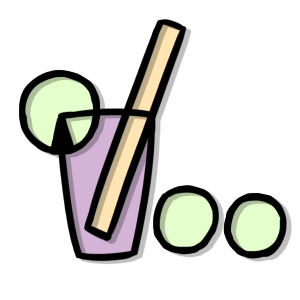
\includegraphics[scale=3]{images/lille_promille_logo.png}    
\end{center}
\thispagestyle{empty}
\newpage
\tableofcontents
\thispagestyle{empty}
\newpage
\setcounter{page}{1}

\section{Begrepsliste}
\begin{tabular}{ | m{4cm} | m{12cm} | } 
    \hline
    \textbf{Begrep} & \textbf{Forklaring} \\
    \hline
    Økt & Perioden fra man drikker sin første enhet til man er kjørbar \\
    \hline
    Kjørbar & At man er i stand til å kjøre bil (Man holder promillegrensen) \\
    \hline
    Enhet & Beskriver en drikke basert på alkoholinnhold og volum \\
    \hline
  \end{tabular}

\section{Introduksjon}
Det er ingen hemmelighet at det festes mye gjennom studietiden og som konsekvens fører dette til at noen velger å fyllekjøre, enten om det er for å komme seg hjemm eller for å ta med festen på veien. Samtidig er det ingen god løsning til dette problemet, selv om loven straffer hardt mot fyllekjøring hindrer det ikke noen prøver seg. Så hvordan kan dette begrenses?

Lille Promille er en app som takler dette problemet ved å fokusere på selve drikkingen. Hvis man kan kontrollere seg selv og sine venner, vil man kunne ta bedre valg og unngå å kjøre i påvirket tilstand. For å gjøre dette, tilbyr appen en oversikt over kjøretilstanden sin. Man får innsikt til alkohol i blodet, antall drikker man har drukket, og hvor lenge det er til man kan kjøre bil. Det vil også være et vennesystem der man kan se hvor mye venner har drukket, som bidrar i å engasjere studenter til å bruke appen.

Appen vil ikke kun være for studenter, men alle som ønsker å ha kontroll mens man fester. Visjonen er at man kommer til å bruke Lille Promille appen for å få oversikt over hvor man drikker, samt hvor mye venner drikker. Det vil være en app som gjør festingen bedre men samtidig minsker sjansen for fyllekjøring, siden dette er av erfaring noe mange lurer på mens de er påvirket.

\section{Hvordan fungerer appen?}
\subsection{Et eksempel}
Ta utgangspunkt i at det er en fest på en søndagskveld, og dagen etter må man være klar til å kjøre til høgskolen tidlig ettermiddagen. Når man tar sin første drikk, åpner man appen og legger til en enhet som passer drikken, for eksempel en rusbrus. Man velger å legge til disse for hver slurk eller for hver flaske man har drukket. Appen vil med jevne mellomrom beregne promillen, slik at man har full oversikt gjennom hele festen. Appen viser rett før midnatt at det er tolv timer til man er kjørbar, og man velger å stoppe å drikke.

Dagen derpå sjekker man appen og ser at det fremdeles er noen venner som er påvirket, og til og med noen som enda drikker. Men siden man følgte appens anvisninger, er man sikrere på at man har beholdt promillegrensen og er klar til å kjøre bil. I tillegg har man muligheten til å se hvordan økten gikk på festen, som hvor man befant seg til diverse tider, hvor mye man drakk og hvor ofte. Disse dataene kan man igjen bruke til senere fester slik at man blir sikrere på sine egne grenser og hva man tåler av alkohol.

\section{Design}

\subsection{Sider i Appen}
\subsubsection{Oversiktsside}
Et av de viktigste stedene i appen er oversiktssiden der all informasjon relatert til en \textit{økt} står oppsummert. Siden består av en nedtellingsklokke, en liste over hva man sist har drukket, og en knapp for å legge til en ny drukket enhet. 

Tanken her er at når brukeren begynner å drikke, legger de til en nydrukket enhet til listen vist på skjermen. I dette øyeblikket starter en ny økt, der nedtellingsklokken viser tiden det vil ta før man er \textit{kjørbar} basert på kjønn, vekt og høyde på brukeren. Dersom brukeren drikker enda en enhet, legges denne til i økten ved hjelp av knappen, og nedtellingen kalkuleres på nytt. Etter hvert som tiden går vil listen på oversiktssiden fylles opp med type enhet som ble konsumert, når den ble konsumert og hvor mye alkohol den inneholder. Under nedtellingsklokken vil det stå en tilnærmet verdi av den nåværende promillen i blodet til brukeren. 

Når nedtellingsklokken har nådd null sekunder, vil økten avsluttes og bruker vil være kjørbar. Denne økten vil derretter bli lagret, slik at man kan inspisere denne økten senere i en egen side med tidligere økter. 

\begin{figure}[H]
    \centering
    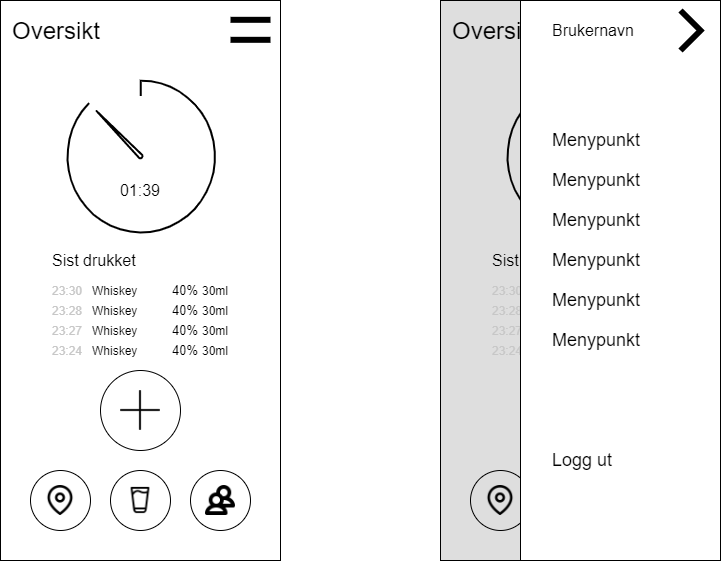
\includegraphics[scale=0.4]{images/lille_promille_frontpage.drawio.png}
    \caption{Til venstre er oversiktssiden med følgende elementer: Nedtellingsklokken, liste av nydrukkede enheter, en pluss-knapp og et navigasjonselement på bunnen. Når man trykker pluss knappen dirigeres man til enhetskatalogen, kan man velge en enhet man vil legge til i økten. Til høyre er det skisset en meny (navigation-drawer i Android studio) med menypunkter som man kan bruke til å navigere appen.}
\end{figure}

\subsubsection{Enhetskatalog}
Enhetskatalogen er en side med opplistning av alle definerte enheter i Appen, og brukes til å legge til enheter i løpet av en økt. Som ny bruker, vil det allerede ligge predefinerte enheter i listen som de kan bruke og gjøre endringer på. Ved behov kan nye enheter bli laget av brukeren gjennom pluss-knappen, da vil det komme opp en modal med noen tekst-felter. Her må brukeren beskrive navn på enheten, alkoholprosent og volum. For eksempel kan man lage en enhet som man kaller for "Whiskey Shot" med 40\% alkohol og 30ml volum. For å slette enheter trykker man på i-symbolet ved siden av navnet, og man blir sendt til en ny side med informasjon om den spesifikke enheten der man kan velge å slette enheten.

\begin{figure}[H]
    \centering
    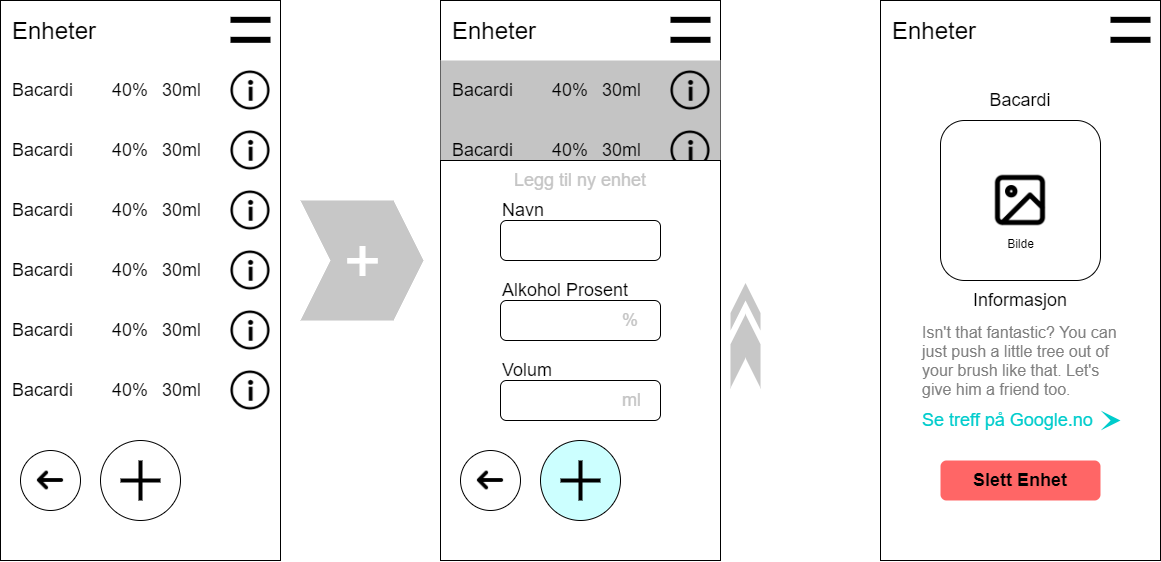
\includegraphics[scale=0.4]{images/lille_promille_unitcatalog.drawio.png}
    \caption{Enhetskatalogen: Listen til venstre består av tidligere definerte enheter. Det er denne siden man benytter når man skal legge til enheter i en økt, og det gjør man ved å trykke på navnet. Med pluss-knappen kan man legge til en ny enhet i listen, og med i-knappen kan man se mer informasjon om enheten. På informasjonssiden har man også valget å slette enheten fra listen.}
\end{figure}

\subsubsection{Innstillinger}
For å endre på noe med kontoen eller med appen går man til siden som heter "innstillinger". Her vil det være listet en rekke innstillinger gruppert etter konto, apputseende og generelle instillinger, som man kan endre på. Disse vil være knyttet opp til den spesifikke brukerkontoen som er logget inn. Når man er fornøyd med endringene sine må man trykke "Lagre endringer" for at de skal ta effekt.

\subsubsection{Venneside}
Vennesiden er der man kan legge til venner og se statusen på venner, som baserer seg på den nåværende økten. Man kan også sende emoji-meldinger til en venn i et chatrom. Dette er for å øke engasjementet ved å la brukerene kommunisere med hverandre, men de må være kreative i prosessen. Det kan bli interessant å se bruken av emojis når man er påvirket av alkoholen. 

\begin{figure}[H]
    \centering
    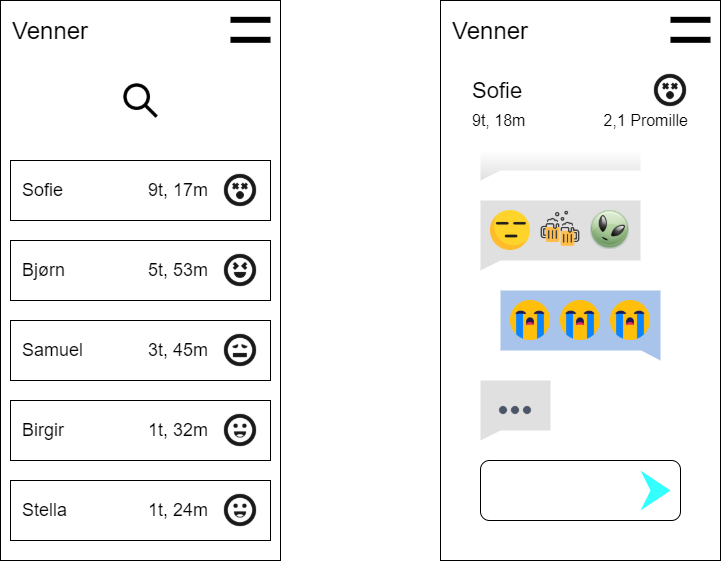
\includegraphics[scale=0.4]{images/lille_promille_friends.drawio.png}
    \caption{Til venstre er listen av venner. Det er tenkt at brukeren kan søke etter venner ved hjelp av forstørrelsesglasset og kunne sende de en venneforespørsel. Til høyre er en skisse av chat-funksjonen, hvor man kan sende emoji-meldinger til en venn. De kan også svare tilbake, og meldingene vil bli vist på siden sortert etter tid.}
\end{figure}

\subsubsection{Kartside}
Appen kommer med en kartside som bruker Google maps API-et. Dersom man er påvirket (En økt har begynt), vil kartet oppdatere hvor man har besøkt i perioden man er påvirket av alkohol. Hensikten med dette er å gi en geografisk oversikt over økten, slik at man vet hvor man har vært mens man drakk. Dette er en funksjon som mange studenter kan ha behov for, siden det ofte hender at de beveger seg rundt når de drikker.

\subsubsection{Innloggingsside}
Dersom man ikke er innlogget, eller man åpner Lille Promille appen for første gang, møter man en innloggingsside. Appen krever enten en e-mail og passord, eller en google-konto for å logge inn. Har man ikke noen av disse, kan man opprette en ny bruker ved å klikke "Opprett bruker" lenken på denne siden, da vil man bli ført til en ny side der man skriver ned en e-mail og et passord. Første gang man logger inn vil Appen spørre om navn, kjønn, vekt og høyde. Navnet er viktig i framvisningen av vennesiden, og de tre siste dataene brukes til beregning av promillen i blodet.

\subsubsection{Økthistorikk og Individuelle Økter}
Ettersom man gjennomgår flere og flere økter, vil de lagres ettersom i en egen historikkside for økter. Her vil man kunne se alle økter sortert etter kronologisk rekkefølge, og man kan inspisere hver individuelle økt ved å klikke på de. Når man gjør dette, åpnes en ny side med informasjon om den spesifikke økten.

\begin{figure}[H]
    \centering
    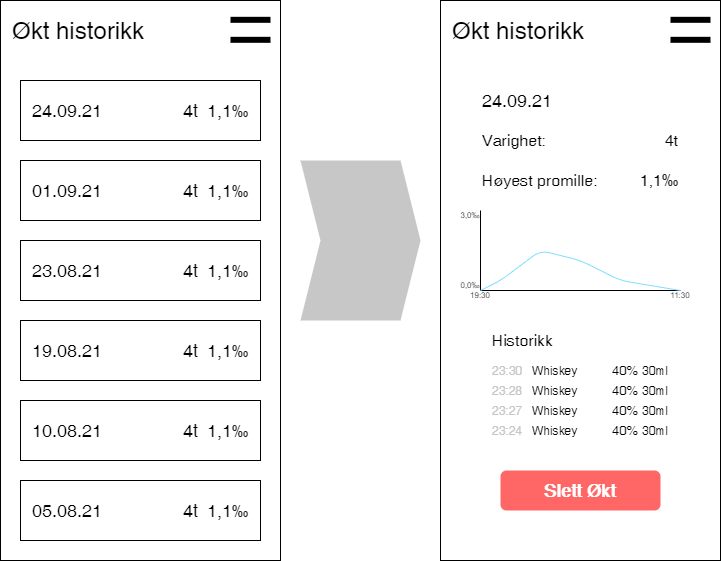
\includegraphics[scale=0.4]{images/lille_promille_sessions.drawio.png}
    \caption{Skisse som viser hvordan økt-historikksiden kan se ut. Her kan man inspisere hver individuelle økt og få utdypet data om hver økt. Det er også mulig å slette en økt.}
\end{figure}

\subsection{Utseende}
Kodeordet for grafikken i Lille Promille er "oversiktlig". Derfor går vi for et rent utseende med få komponenter i hver side, slik at det ikke blir for mye rot. Hensikten er at man ønsker gjerne kun den relevante informasjonen i en slik app, spesielt når man er påvirket av alkohol. Nedtellingsklokken på forsiden er ganske stor for å fange oppmerksomheten, og videre er informasjon vist i rekkefølge nedover siden basert på viktighet. Dette design-prinsippet følger stort sett alle sider i appen for å gjøre opplevelsen mest behagelig som mulig for brukeren. Skjermbildene ovenfor demonstrerer dette.

Fargemessig har vi gått for nøytrale farger, med noe rødt og blått for å signalisere funksjonaliteten til brukeren. For eksempel en rød knapp for å signalisere at noe skal slettes, eller en blå tekst for å markere at den er interaktiv.

Videre har vi valgt å gruppere og abstrahere informasjon vekk fra første-sidene, slik at man ikke overvelder brukeren med informasjon. Et godt eksempel på dette er økt-historikken, da man kan velge å inspisere en spesifikk økt for å se mer informasjon om den økten. Dette er også et prinsipp som går gjennom hele appen. Appen benytter seg også av ikoner for å dirigere bruker i riktig retning og gi mer kontekst bak de interaktive elementene.

\subsection{Navigasjon}
Appen består av to hovedelementer for navigasjon, et bottom-navigation element, og et navigation-drawer element. I tillegg til disse har den en swipe-funksjon når man befinner seg i forsiden, kartsiden og vennesiden. Det vil være mulig å navigere mellom disse tre sidene med bottom-navigation elementet, men også å swipe fra venstre til høyre og motsatt. Tilgjengelig fra de fleste sider vil være en navigation-drawer som brukes til å navigere til resten av appen.

Grunnen til denne oppdelingen er for å skille mellom sider som blir brukt mye og sider som blir brukt lite. Vi har valgt å bruke bottom-navigation og swipe-funksjonen til forsiden, kartsiden og vennesiden, fordi de er sentrale og brukes nesten hver gang appen er i bruk. Forsiden er det samme som oversiktssiden, så dette vil være landingssiden når brukeren logger inn. I navigation-drawer elementet kan man blant annet navigere seg til innstillinger og enhetskatalogen.

    \subsubsection{Flyt}

    \begin{figure}[H]
        \centering
        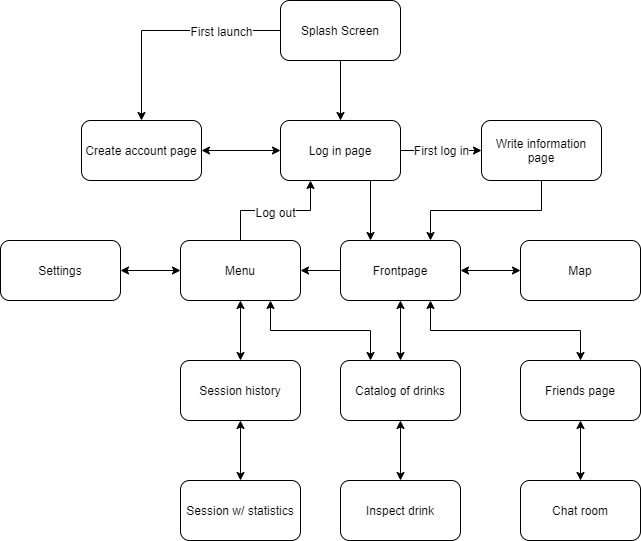
\includegraphics[scale=0.5]{images/lille_promille_float_diagram.drawio.png}
        \caption{Skisse som viser hvor man kan navigere seg til fra hvilke sider i appen.}
    \end{figure}

    \subsubsection{Navigation Pattern}
    Bla bla bla

\subsection{Teknisk oppbygging}
Blablabla

    \subsubsection{Lagring og uthenting av data}
    Blablabla

    \subsubsection{Brukerhåndtering}
    I am blue
    Da ba de da ba die

\section{Krav}
\freq{Bruker skal kunne oppgi informasjon om sin vekt, kjønn og høyde} 
\freq{Bruker skal kunne opprette en brukerkonto}
\freq{Bruker skal kunne logge inn med eksisterende brukerkonto}
\freq{Bruker skal kunne starte og stoppe en økt}
\freq{Brukeren skal kunne legge til en enhet til nåværende økt}
\freq{Appen skal kunne kalkulere nåværende promille basert på vekt, kjønn og høyde}
\freq{Appen skal kontinuerlig vise nåværende promille}
\freq{Appen skal kunne vise når man kan kjøre basert på nåværende promille}
\nfreq{Appen skal opprettholde kontraststandard i forhold til WCAG 2.0}
\freq{Bruker skal kunne slette tilhørende brukerkonto}
\freq{Bruker skal kunne inspisere tidligere økter med vedlagt statistikk}
\freq{Bruker skal kunne slette tidligere økter}
\freq{Brukeren skal kunne legge til sin egendefinerte enhet til den eksisterende listen av enheter}
    \fsubreq{Brukeren skal kunne bestemme volum, prosentandel og navn på den nye enheten}
\freq{Brukeren skal kunne fjerne enheter fra den eksisterende listen av enheter}
\freq{Appen skal kunne arkivere økter (dvs. antall enheter)}
\freq{Appen skal kunne spore mobilen for hver økt}
\freq{Appen skal kunne loggføre statistikk}
\freq{Appen skal vise nedtellingen på lock-screen på telefonen}
\freq{Bruker skal kunne slå av og på sporing av mobilenheten}
\freq{Appen skal vise en venneliste}
\freq{Bruker skal kunne legge til nye venner i vennelisten}
\freq{Bruker skal kunne sende en emoji-melding til en spesifikk venn}
\freq{Appen skal vise promille-status for hver venn ved siden av navnet deres}
\nfreq{Brukeren skal kunne velge mellom darkmode eller lightmode}
\nfreq{Brukerene skal varlses dersom drikken de søker etter ikke er i listen}
\freq{Bruker skal valgfritt kunne oppgi alder}
\freq{Bruker skal kunne velge “glemt passord” etter behov}
\freq{Appen skal kunne tilbakestille passord til bruker etter forespørsel}
\freq{Bruker skal kunne endre på alle opplysninger på tilhørende brukerkonto}
\freq{Bruker skal kunne oppgi klokkeslett for når man ønsker å være kjørbar}
\freq{Bruker skal kunne oppgi maksimal promille som ikke skal overstiges}
    \fsubreq{Appen skal kunne varsle at bruker har nådd maksimal promille}
\freq{Bruker skal kunne oppgi maksimal antall enheter som skal konsumeres}
\freq{Brukeren må samtykke til vilkår for bruk før de kan bruke appen}
\freq{Appen skal kunne detektere om brukeren kjører mens de er påvirket}
    \fsubreq{Appen skal kunne varsle at bruker kjører}
\freq{Appen skal kunne vise en statusbar som viser brukerens status}
\freq{Appen skal kunne vise hvordan promillen endret gjennom økten seg basert på når en enhet ble konsumert}
\freq{Appen skal kunne varsle at bruker bør drikke vann}
\freq{Bruker skal kunne bestemme om appen skal varsle at de bør drikke vann}
\freq{Bruker skal kunne velge å bli varslet etter hver drukket enhet, eller ved en terskel}
\freq{Appen skal kunne vise åpningstider til barer}
    \fsubreq{Appen skal kunne finne nærmeste bar}
    \fsubreq{Brukeren skal kunne ha mulighet til å filtrerer barer på aldersgrenser}
\freq{Appen skal gjøre det mulig å ta bilde av etikken på flasken for å legge til en enhet}
\freq{Brukeren skal kunne se oppskrifter på drinker}
\freq{Brukeren skal kunne sjekke koordinasjonen basert på sensorer}

\end{document}